%Einleitungstext zum Modul
Der Logger verwendet die Biblothek QsLog und stellt Funktionalitäten für die GUI bereit.
\section{Klassen}
\graphicspath{{./img/logger/}}
%Bild der Klasse aus dem Klassendiagramm (nur die Klasse jeweils)
%Dokumentation zur Klasse, öffentlichen Methoden und Konstruktor sowie:
%Signal und Slots als Methoden mit Rückgabewert Sigal bzw Slot (zur kenntlichkeit) 
\subsubsection{CLogInit}\label{Logger: CLogInit}
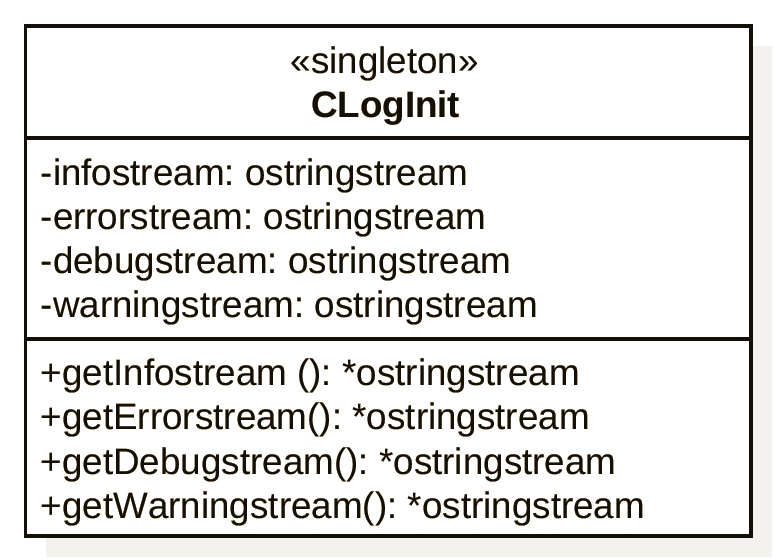
\includegraphics[scale=0.4, resolution=100]{cloginit}\\
Initialisierungsklasse für den Logger erzeugt bei Objekterzeugung die  otextstream-Objekte und gibt über die Schnittstellen Objektreferenzen weiter. 
\beginAttributes
\newAttribute{private infostream}{Objekt Referenz auf das otextstream-Objekt zum loggen der Infonachrichten}
\newAttribute{private errorstream}{Objekt Referenz auf das otextstream-Objekt zum loggen der Errornachrichten}
\newAttribute{private debugstream}{Objekt Referenz auf das otextstream-Objekt zum loggen der Debugnachrichten}
\newAttribute{private warningstream}{Objekt Referenz auf das otextstream-Objekt zum loggen der Warningnachrichten}
\closeMembers
\beginMembers
\newMember{{ClogInit}}{void}{void}{Konstruktor: erzeugt 4 otextstreamobjekte und speichert diese ab}
\newMember{{getInfostream}}{void}{otextstream}{Gibt eine Objektreferenz auf das Infostream Objekt zurück}
\newMember{{getErrorstream}}{void}{otextstream}{Gibt eine Objektreferenz auf das Errorstream Objekt zurück}
\newMember{{getDebugstream}}{void}{otextstream}{Gibt eine Objektreferenz auf das Debugstream Objekt zurück}
\newMember{{getWarningstream}}{void}{otextstream}{Gibt eine Objektreferenz auf das Waningstream Objekt zurück}
\closeMembers





\subsection{CLogController}\label{Logger: CLogController}
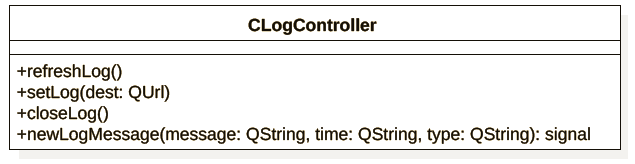
\includegraphics[scale=0.8, resolution=100]{clogcontroller}\\
Überprüft die otextstream-Objekte und stellt das Bindeglied zwischen der QSLog Biblothek, GUI und otextstream Objekte da. 
\beginMembers
\newMember{{refreshLog}}{void}{void}{Überprüft die otextstreamobjekte auf neue Nachrichten ud gibt diese an die GUI(per Signal) an den QSLogger und an die History weiter}
\newMember{{setLog}}{dest : QString}{void}{setzt den Datenpfad für ein Log auf den momentanen Ergebnissordner. Muss beim Start des Algorithmendurchlaufs gesetzt werden}
\newMember{{closeLog}}{void}{void}{schließt das aktuelle Log ab. Muss nach Ende des Algorithmendurchlaufs ausgeführt werden}
\closeMembers
\beginSignals
\newSignal{newLogMessage}{message: QString, time: QString, type: QString}{Wird aufgerufen, wenn eine neue Lognachricht vorhanden ist}
\closeMembers
\subsection{CLogHistory}\label{Logger: CLogHistory}
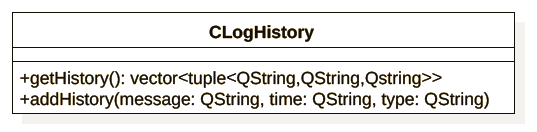
\includegraphics[scale=1, resolution=100]{cloghistory}\\
temporäre History der Log Nachrichten für die Oberfläche 
\beginMembers
\newMember{{addHistory}}{message: QString, time: QString, type: QString}{void}{fügt neue Lognachrichten der History hinzu mit Nachricht, Zeit, Typ der Nachricht}
\newMember{{getHistory}}{}{<vector<tuple<Qstring,QString,QString>>}{gibt die momentane History zurück mit Nachricht,Zeit,Typ der Nachricht als Vektor zurück}
\closeMembers
\subsection{QsLog}\label{Logger: QsLog}
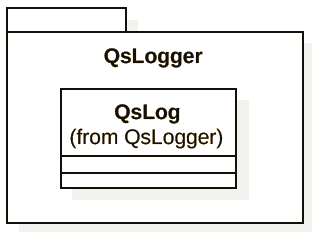
\includegraphics[scale=0.9, resolution=100]{qslog}\\
Die QsLog Bibliothek stellt einen Logger bereit der durch CLogInit initialisiert und durch CLogController verwedendet wird um Log Dateien zu füllen.Weitere Erläuterungen: siehe Paket QsLog

\subsection{otextstream}\label{Logger: otextstream}
%\includegraphics[scale=1, resolution=100]{}\\
Standard C++ Klasse die verwendet wird um 4 einfache Streamobjekte zu verfügung zu stellen, in welche die Algorithmen Plugins ihre Nachrichten schreiben können.
\section{Pakete}
%Einteilung der Teilmodule in Pakete 
\subsection{QsLog}
%Bild des Pakets mit vereinfachter Klassendarstellung
%Begründung / Dokumentation / Erklärung zum Paket
QsLog Bibliothek zur Speicherung der Logs auf der Festplatte.
QsLog biete 6 Loglevel und ist Thread-safe. Es ist eine einfach zu nutzende Bibliothek.
QsLog kann in Projekten mit MIT oder strengeren Lizenzen verwendet werden und muss ensprenchend gekennzeichnet werden.
Weitere Informationen und Quellcode sowie Dokumentation ist auf github.com/victronenergy/QsLog zu finden.
\subsection{LogController}
Stellt das Bindeglied zwischen den Algorithmen und der QsLog Bibliothek bereit.
Stellt Log Funktionalitäten für die GUI bereit und speichert die Nachrichten temporär für die GUI ab.
%....
\section{Entwurfsmuster}
<Singleton>
\\die Klasse CLogInit stellt ein Singleton dar. Sie darf nur einmal erzeugt und verwendet werden.
\\<Adapter>
\\Die Klasse CLogController stellt einen Adapter zwischen den otextstream Objekten und den Streamobjekten der QsLog Bibliothek dar.
\newpage
\section{Klassendiagramm}
%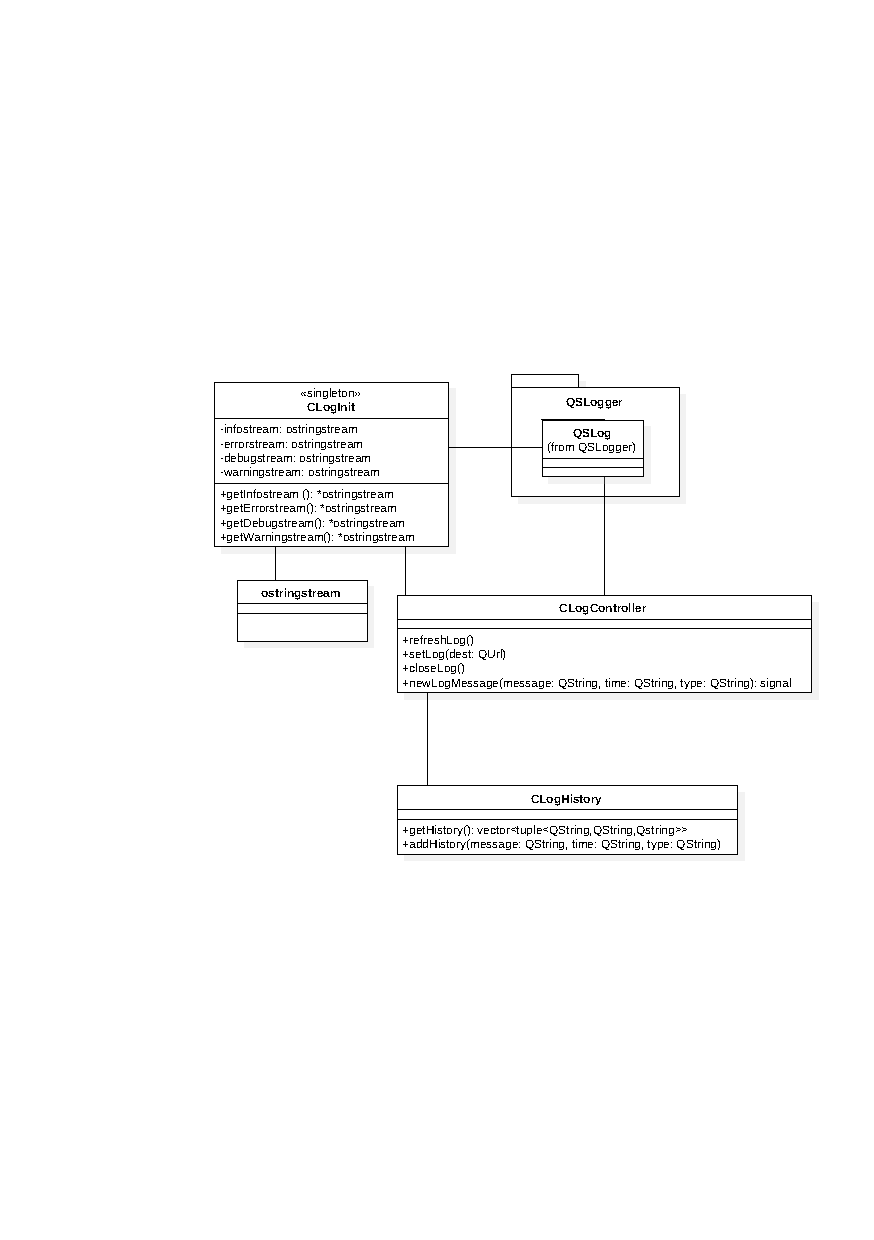
\includegraphics[width=\linewidth]{Klassendiagramm}
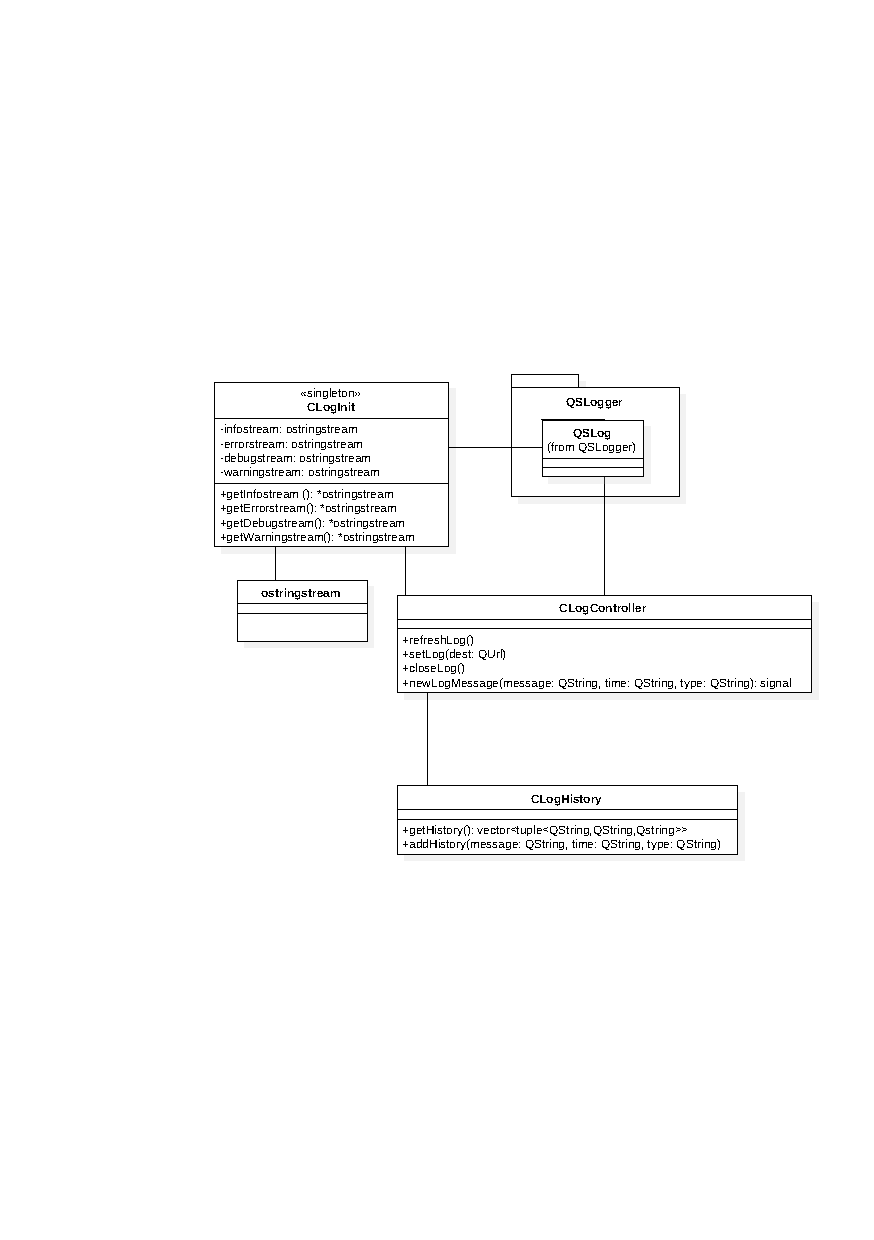
\includegraphics[scale=0.6]{Klassendiagramm.pdf}
%Bitte jeweils kleine Einleitungstexte usw in Unterkapitel gerne auch in Textform Erklärungen zufügen und auf mögliche erweiterungen durch die kann Kriterien eingehen soweit nötig !